% TO-DO:
% * Actions = all possible transtions in RL
% * In RL, Q-learning is still unclear -- currently I'm using NN = transition F(x)
%   -- U(x) -> U(x') so it seems that generalization can occur in Q-space (?)
% * Structure of the turnstile is an important feature of the transition F(x)
% * Explain difference with AIXI
% * "inward" vs "outward"

\documentclass[orivec]{llncs}
\usepackage{graphicx}
\usepackage{float}
\usepackage[most]{tcolorbox}% for wrapping example in color box
\usepackage{wrapfig}		% wrap figure beside text, used in example
\usepackage{tikz-cd}		% commutative diagrams
% \usepackage{amsfonts}
\usepackage[normalem]{ulem}	% underline with line breaks: /uline
\usepackage{enumitem}       % for using (A),(B),(C) in items...
\usepackage{amsmath}		% for "cases"
\usepackage{amsfonts}		% for frakur fonts
\usepackage{mathrsfs}		% for curly "E" error symbol
\usepackage{amssymb}		% for \multimap, \updownarrow, \bigstar
\usepackage{turnstile}		% longer turnstiles
\usepackage{sectsty}		% change section color
\usepackage{hyperref}		% refs, links become clickable
\usepackage{url}			% for urls in bibliography
\usepackage[normalem]{ulem} % underline unbroken with \uline
\usepackage[numbers,sectionbib]{natbib}% if we use \package{url} we need to use natbib style

%\def\chinchin{yes}          % ********** 用中文 *********
% *************** Delete when not using Chinese or colors **********************
\ifdefined\chinchin
	\usepackage{xeCJK}
	\setCJKmainfont[BoldFont=SimHei,ItalicFont=KaiTi]{SimSun}
\fi
\usepackage{color}
%\newcommand{\emp}[1]{\textbf{\textcolor{blue}{#1}}}
\newcommand{\emp}[1]{\textbf{#1}}

\sectionfont{\color{blue}} 
\subsectionfont{\color{blue}} 
\subsubsectionfont{\color{blue}} 
\definecolor{green}{rgb}{0,0.7,0}
\definecolor{grey}{rgb}{0.95,0.95,0.95}

\usepackage{geometry}		% change paper size
\geometry{
  a4paper,         % or letterpaper
  textwidth=18cm,  % llncs has 12.2cm
  textheight=27cm, % llncs has 19.3cm
  heightrounded,   % integer number of lines
  hratio=1:1,      % horizontally centered
  vratio=2:3,      % not vertically centered
}
\usepackage[fontsize=13pt]{scrextend}

\newcommand{\tikzmark}[1]{\tikz[overlay,remember picture] \node (#1) {};}

\newcommand{\vect}[1]{\boldsymbol{#1}}
\newcommand*\sigmoid{\vcenter{\hbox{
\includegraphics{sigmoid.png}}}}
\newcommand*\rectifier{\vcenter{\hbox{\includegraphics{rectifier.png}}}}
\newcommand*\KB{\vcenter{\hbox{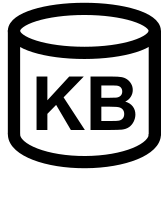
\includegraphics{KB-symbol.png}}}}
\newcommand*\KBsmall{\vcenter{\hbox{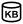
\includegraphics{KB-symbol2.png}}}}
\newcommand*\Eye{\vcenter{\hbox{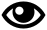
\includegraphics{../eye-symbol.png}}}}
\newcommand*\NN{\vcenter{\hbox{
\includegraphics{NN-symbol.png}}}}
\newcommand*\Graph{\vcenter{\hbox{\includegraphics{../graph-symbol.png}}}}
\newcommand*\Hypergraph{\vcenter{\hbox{\includegraphics{../hypergraph-symbol.png}}}}
\newcommand*\Tree{\vcenter{\hbox{\includegraphics{../tree-symbol.png}}}}
\newcommand*\NewSym[1]{\vcenter{\hbox{\includegraphics{#1}}}}
\newcommand{\dashh}{\textemdash~}
\newcommand{\english}[1]{\mbox{\textit{#1}}}
\newcommand{\tab}{\hspace*{2cm}}

% ***** Boxed variables inside math equations
% \newcommand*{\boxedcolor}{black}
\makeatletter
% \renewcommand{\boxed}[1]{\textcolor{\boxedcolor}{%
% \fbox{\normalcolor\m@th$\displaystyle#1$}}}
% \setlength{\fboxsep}{1pt}
\renewcommand{\boxed}[1]{\fbox{\m@th$\displaystyle\scalebox{0.9}{#1}$} \,}
\makeatother

\overfullrule=0mm

\newsavebox{\MyName}
\savebox{\MyName}{
\includegraphics[scale=0.6]{YKY.png}}

\title{
\ifdefined\chinchin
神经网络中的「内省」\\
(``introspection'' in neural networks)
\else
``Introspection'' in neural networks
\fi
}
%\normalsize{-- a minimalist cognitive architecture combining\\
%reinforcement learning and deep learning}}
\titlerunning{Introspection}
\author{\usebox{\MyName} (King-Yin Yan)
% \\ \footnotesize{General.Intelligence@Gmail.com}
%\and
%Ben Goertzel
%\and
%Juan Carlos Kuri Pinto
}
\institute{General.Intelligence@Gmail.com}
\date{\today}

\begin{document}
\let\labelitemi\labelitemii

\maketitle

\noindent
\makebox[\linewidth]{\small \today}

\setlength{\parindent}{0em}
\setlength{\parskip}{2.8ex plus0.8ex minus0.8ex}
% \setlength{\parskip}{2.8ex}

\begin{abstract}
\ifdefined\chinchin
在本文中「内省」是指智能系统直接读/写知识的能力,此能力在经典 logic-based AI 是免费做到的,但神经网络内的「知识」素来有「黑盒」的问题。  解决办法是让神经网络直接作用在它自身的 weights 上。  
\else
In this paper, ``introspection'' refers to the ability of an intelligent agent to access its own knowledge.  This ability comes for free in classical logic-based AI, but neural networks are notorious for the ``black-box'' problem.  The solution is to have the network act on its own weights.
\fi
\end{abstract}

%\begin{keywords}
%reinforcement learning, control theory, deep learning, cognitive architecture
%\end{keywords}

\setcounter{section}{-1}
\section{Introduction}
% \label{sec:0}

\ifdefined\chinchin
这篇文章说的「内省」的意思是指智能系统有能力读/写它内部的知识。  例如说,一个比较蠢的智能系统可以用 sequence-to-sequence 的方式将中文翻译成英文: 
\begin{equation}
\mbox{``}\boxed{中文句子}\mbox{''} \stackrel{\vect{F}}{\longrightarrow} \mbox{``}\boxed{英文句子}\mbox{''}
\end{equation}
\else
By ``introspection'' is meant the ability of an intelligent agent to \textbf{access} (read or write) the contents of its knowledge base.  For example, a dumber agent may use the ``sequence-to-sequence'' technique to translate Chinese sentences into English:
\begin{equation}
\mbox{``}\boxed{Chinese sentence}\mbox{''} \stackrel{\vect{F}}{\longrightarrow} \mbox{``}\boxed{English sentence}\mbox{''}
\end{equation}
\fi
\ifdefined\chinchin
$\vect{F}$ 代表系统的函数。  但系统并不真的明白句子的意义,句子只是「水过鸭背」地流过系统。 一个更聪明的系统是: 句子可以\textbf{进入}到 $\vect{F}$ 里。 我所说的「内省」就是这意思。
\else
$\vect{F}$ is the system's \textbf{function}.  But the system does not truly understand the sentences' meaning;  The sentences simply ``pass through'' the system.  A more intelligent agent would allow sentences to \textbf{go into} $\vect{F}$.  This is what I mean by ``introspection''.
\fi

\ifdefined\chinchin
「内省」亦有 meta-reasoning 的意思,亦即除了\textbf{外在}的知识,系统还拥有关於系统\textbf{自身状态}的知识。 但本文中「内省」是指存取「普通知识」的能力。
\else
``Introspection'' also connotes \textbf{meta-reasoning}, which means that, in addition to \textbf{extrinsic knowledge}, the system also possesses knowledge about \textbf{its own states}.  In this paper, we only concern ourselves with the agent's access to extrinsic knowledge.
\fi

\section{Applications}

Introspection (in the present paper's sense) is useful in:
\begin{itemize}
	\item learning by instructions, or ``learn by being told'' \\
	(a technique crucial to accelearating the learning of human knowledge)
	\item belief revision / truth maintenance \\
	(the most challenging and highest-level task in logic-based AI)
\end{itemize}

\ifdefined\chinchin
举例来说,小孩子的行为是由他内部的知识决定的,「知识决定行为」。
\begin{itemize}
	\item 当小孩子看到一个成人做的动作,他会模仿那动作。
	\begin{equation}
	\vcenter{\hbox{
\includegraphics[scale=0.5]{imitation.jpg}}}
	\end{equation}
	\item 或者小孩子听到一句说话:「不要吃污糟食物」,他明白了那句说话的意思而改变行为。
\end{itemize}
\else
For example, a child's behavior is determined by his internal knowledge; ``Knowledge determines action''.
\begin{itemize}
	\item When a toddler watches an adult's gesture, he tries to imitate that gesture:
	\begin{equation}
	\vcenter{\hbox{
\includegraphics[scale=0.5]{imitation.jpg}}}
	\end{equation}
	\item Or when a child hears a saying:  ``don't eat dirty food'', he understands the words and changes his behavior.
\end{itemize}
\fi
\ifdefined\chinchin
这两个例子都涉及到将「感觉资料」放进 $\vect{F}$ 里面:
\else
Both examples involve putting ``sensory data'' into $\vect{F}$:
\fi
\begin{equation}
\boxed{sensory data} \hookrightarrow \vect{F}
\end{equation}

\section{Cartesian closure}

Introspection requires the functional closure $\mathbb{X} \simeq \mathbb{X}^{\mathbb{X}}$ which yields a \textbf{Cartesian-closed category} (CCC).

\ifdefined\chinchin
举例来说,「吃了污糟的食物会肚痛」是一个句子,它经由 $\Eye$ 进入 mental state $\vect{x}$ ,变成 proposition。 但我们希望这逻辑命题变成 $\KB$ 的一部分。 
\else
For example, ``eating dirty food causes stomach pains'' is an NL sentence, it enters from $\Eye$ into the mental state $\vect{x}$, as a \textbf{proposition}.  But we want $\vect{x}$ to become part of $\KB$.  
\fi
$\vect{F}$ is the state-transition function:
\begin{equation}
\vect{x}_{n+1} = \vect{F}(\vect{x}_n)
\end{equation}
where \\
\tab $\vect{F} = \KB = \NN$ \\
\tab $\vect{x} = $ state

An individual logic rule is a \uline{restriction} of $\vect{F}$ to a specific input;  Perhaps I could call such elements ``micro-functions''.

$\vect{F} \equiv \KB$ is the \uline{``union'' of micro-functions}:
\begin{equation}
\KB = \bigcup \vect{f}_i
\end{equation}
Or, in a vague sense, $\vect{F}$ is the sum total of objects like $\vect{x}$:
\begin{equation}
\vect{F} = \bigcup \vect{x}_i
\end{equation}
\ifdefined\chinchin
但 $\vect{F}$ 是一个神经网络,它的一般形式是:
\else
But $\vect{F}$ is a neural network;  Its general form is:
\fi
\begin{equation}
\boxed{output} \; \vect{x}_{n+1} = \vect{F}(\vect{x}_n) = \sigmoid \stackrel{1}{W} \; \sigmoid \stackrel{2}{W} \; ..... \; \sigmoid \stackrel{L}{W} \; \vect{x}_n
\end{equation}
$L$ = total number of layers.  
\ifdefined\chinchin
由於各层的非线性「纠缠在一起」,表面上无法将神经网络「分解」。 直到笔者受了 David Ha \textit{et al} 提出的 PathNet \citep*{Fernando2017} 理论所启发,PathNet 是由一些较小的神经网络 modules 组成,所以或许可以建构如下形式的「丝状神经网络」:
\else
Because all the layers of non-linearities are ``entwined together'', apparently we cannot ``decompose'' a neural network.  That is, until the author hears of David Ha \textit{et al}'s PathNet \citep*{Fernando2017} idea, which is a big network consisting of smaller neural-network modules.  Inspired by that, I propose to construct a ``threaded'' neural network:
\fi
\begin{equation}
\vcenter{\hbox{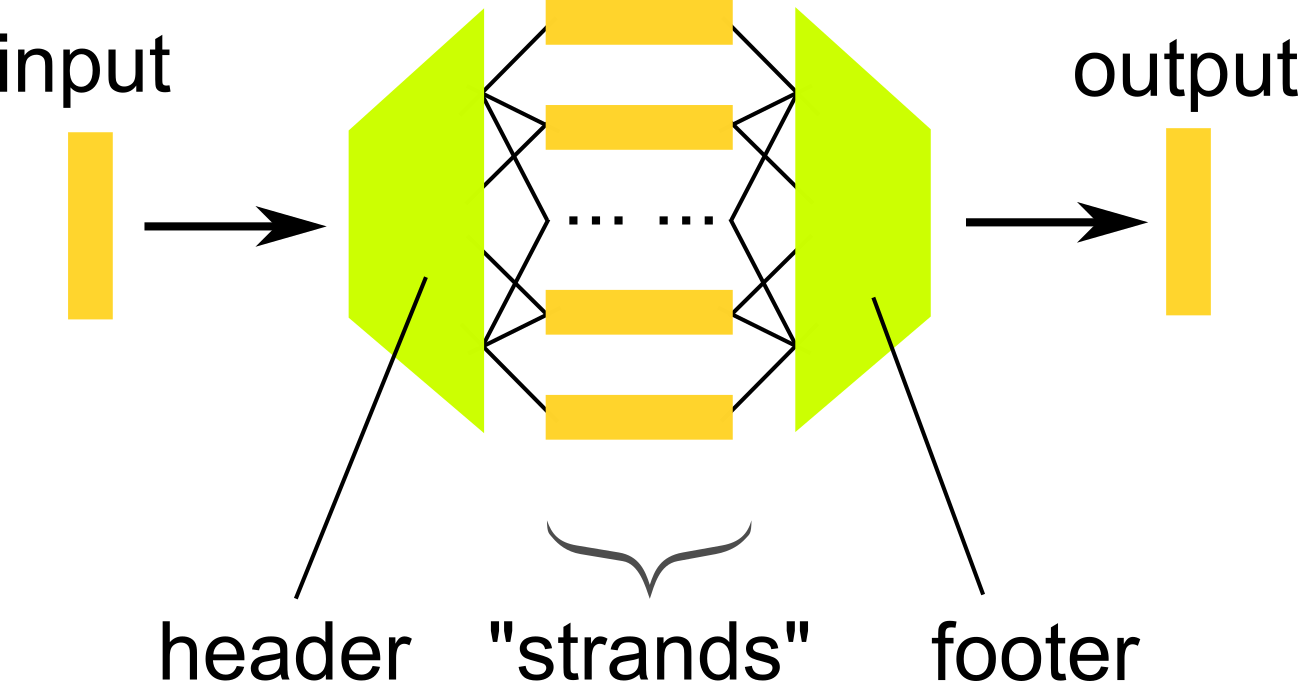
\includegraphics[scale=0.75]{reticular-NN.png}}}
\end{equation}
\ifdefined\chinchin
这些「丝条 $\NewSym{strand.png}$」可以是简单的神经网络,例如每个的宽度或深度很小,因而可以用较短的 weights vector 描述。  正是因为这原因,一个 $\NewSym{strand.png}$ 本身可以作为神经网络的输入。 但整个神经网络 $\vect{F}$ \uline{无法输入自己},因为根据 Cantor's theorem,$\mathbb{X} = \mathbb{X}^{\mathbb{X}}$ 是不可能的。
\else
These ``strands'' $\NewSym{strand.png}$ are simpler neural networks, for instance with smaller widths and depths, so they can be described by shorter weight vectors.  Precisely for this reason, a  $\NewSym{strand.png}$ can be presented as input to its own neural network.  We  \uline{cannot pass the entire network $\vect{F}$ to itself}, due to Cantor's theorem, which says $\mathbb{X} = \mathbb{X}^{\mathbb{X}}$ is impossible.
\fi

Let $\overline{\vect{F}} = \NewSym{header.png} $ header, $\underline{\vect{F}} = \NewSym{footer.png} $ footer, $\vect{f}_i = \NewSym{strand.png}$ strands, then:
\begin{equation}
\vect{F} = \overline{\vect{F}} \circ \bigcup \vect{f}_i \circ \underline{\vect{F}}
\end{equation}
\ifdefined\chinchin
每个 $\NewSym{strand.png}$ 大约对应於逻辑上的一个\textbf{命题}(proposition, 可以是条件命题或普通命题)。
\else
Each $\NewSym{strand.png}$ roughly corresponds to a single \textbf{proposition} in logic-based AI. Such propositions may be conditional or plain statements.
\fi

\begin{equation}
\Theta \in \NewSym{bbTheta.png}
\end{equation}
\begin{equation}
\vcenter{\hbox{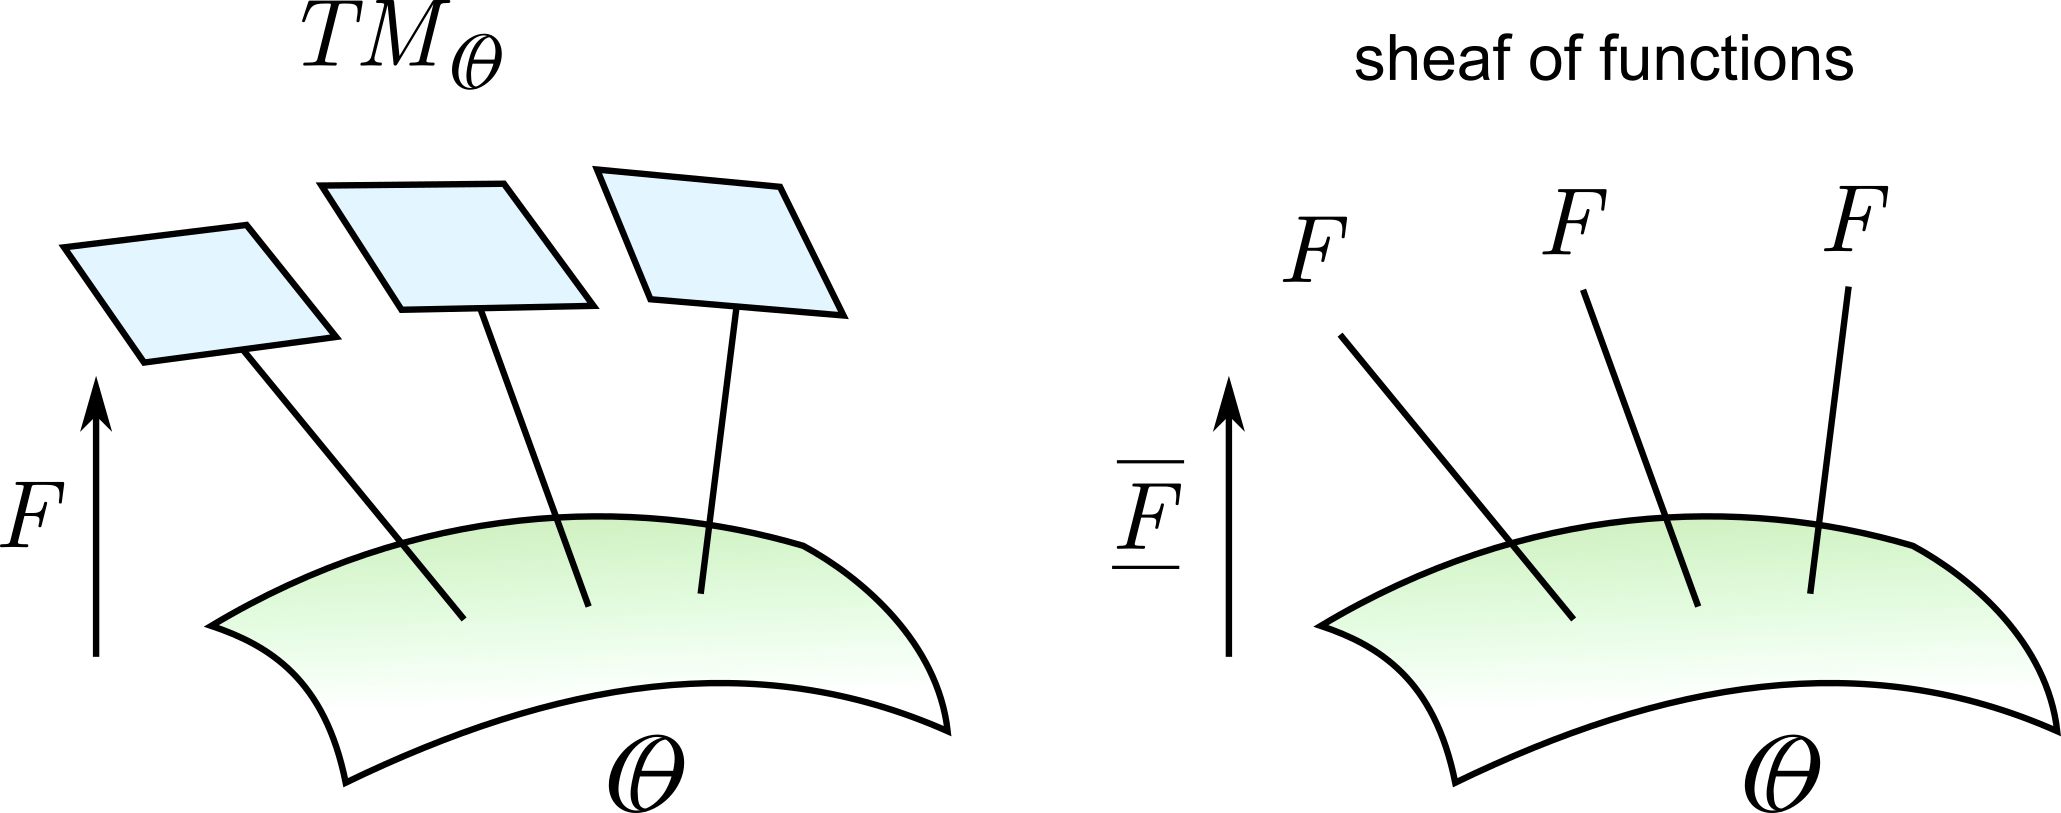
\includegraphics[scale=0.6]{tangent-bundle-and-sheaf.png}}}
\end{equation}


\section{Overall architecture}

For reference, the architecture for \textbf{visual recognition} is:
\begin{equation}
\vcenter{\hbox{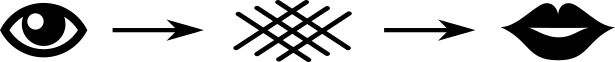
\includegraphics[scale=0.6]{vision-architecture.png}}}
\end{equation}
Our basic AGI architecture is:
\begin{equation}
\vcenter{\hbox{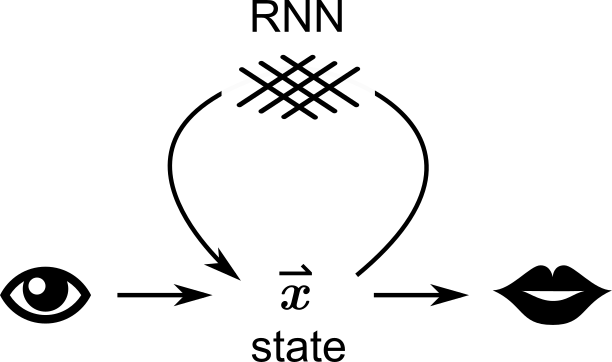
\includegraphics[scale=0.6]{basic-architecture.png}}}
\label{basic-arch}
\end{equation}

$\NN$ = [deep] neural network, trained via \textbf{reinforcement learning}

The overall \textbf{recurrent} setup operates like this:
\begin{equation}
\vcenter{\hbox{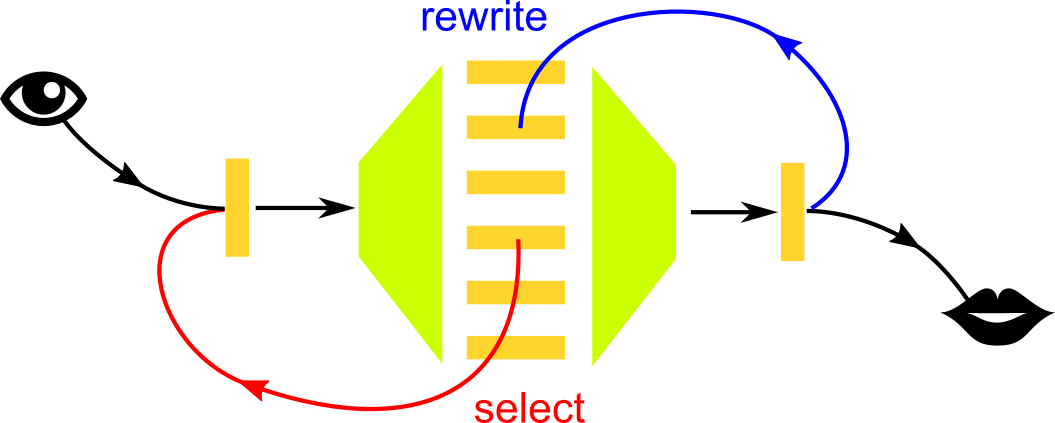
\includegraphics[scale=0.7]{introspection-simple.png}}}
\end{equation}

Viewing the ``information flow'' in a simplified way, we notice a ``second'' pass through the network's internal weights:
\begin{equation}
\vcenter{\hbox{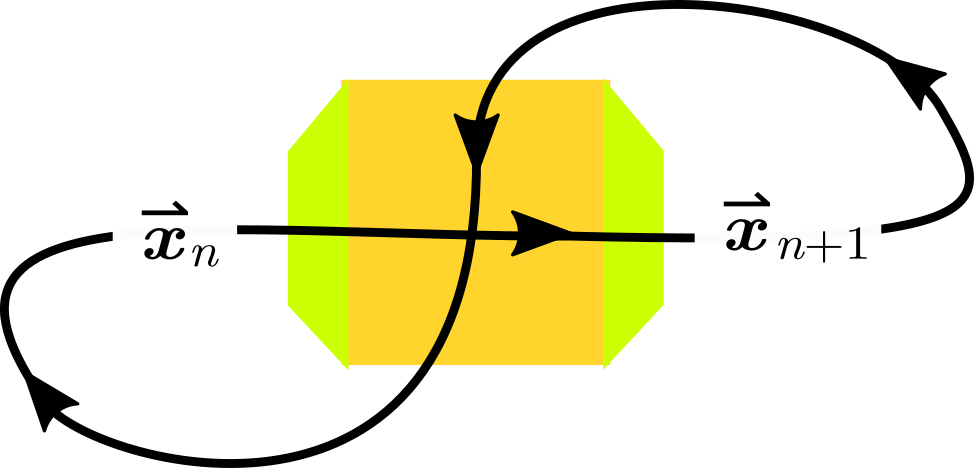
\includegraphics[scale=0.5]{introspection-flow.png}}}
\end{equation}
This mode of operation has always been standard in logic-based systems.  The $\NewSym{IRNN.png}$ is the $\KB$.  The vertical pass represents reading/writing information to/from $\KB$.  The horizontal pass represents using the $\KB$ for logical inference (thinking), ie:
\begin{equation}
\vect{x}_n  \cup \KB \sststile{}{} \vect{x}_{n+1}
\end{equation}

\section{Structure of memories}

The ``main memory'' $\vect{F}$ can take the form of a tree ($\Tree$), graph ($\Graph$), or hyper-graph ($\Hypergraph$), with increasing complexity.

The \textbf{mental state} $\vect{x}$, or ``working memory'', can also assume the above-mentioned forms.

Currently I am not sure whether to place \textbf{episodic memory} inside $\vect{F}$ or as a separate module outside $\vect{F}$.

We need to organize the $\NewSym{strand.png}$'s in the form of $\Tree$, $\Graph$ or $\Hypergraph$, in such a way that the resulting structure is also a neural network, or more generally a mathematical \textbf{function} in Hilbert space.

But there is one simple way:  Basically, a deep network is automatically ``tree-like'' because of its many layers (\textbf{levels}) of weights organized hierarchically.  Thus we can build a network like this:
\begin{equation}
\vcenter{\hbox{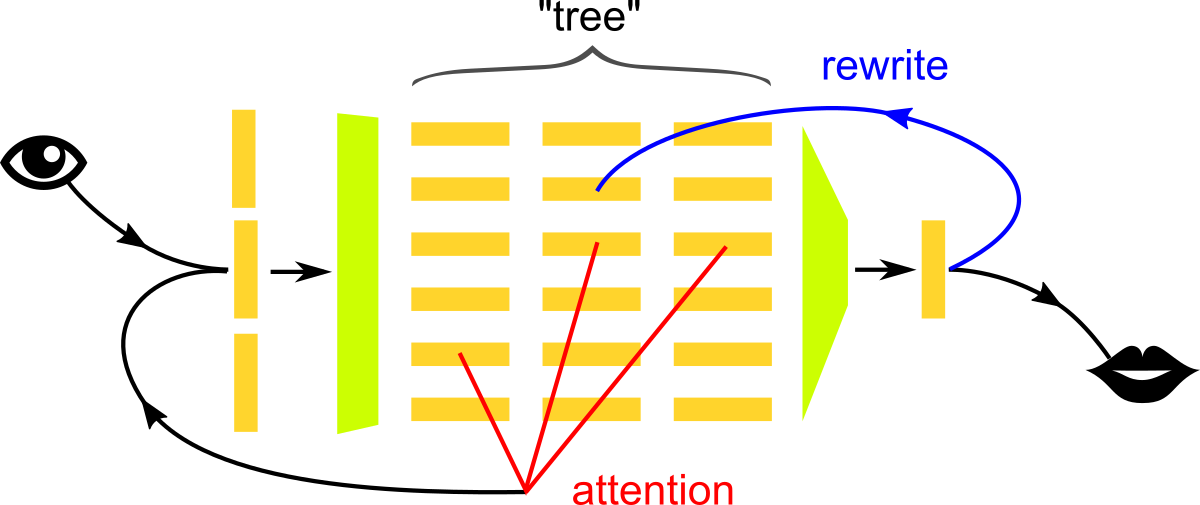
\includegraphics[scale=0.7]{introspection-tree-bank.png}}}
\end{equation}
The {\color{red}attention mechanism} selects a number of $\NewSym{strand.png}$'s to be the \textbf{current state} or ``working memory''.  Notice that the input size is bigger than the output size, which reflects the structure of the logical \textbf{consequece operator} $\vdash$.

\section*{Acknowledgements}

Thanks to David Ha for his PathNet idea.

\bibliographystyle{unsrtnat} % or number or aaai ...
\bibliography{AGI-book}

\end{document}
